%%%%%%%%%%%%%%%%%%%%%%%%%%%%%%%%%%%%%%%%%
% Thin Sectioned Essay
% LaTeX Template
% Version 1.0 (3/8/13)
%
% This template has been downloaded from:
% http://www.LaTeXTemplates.com
%
% Original Author:
% Nicolas Diaz (nsdiaz@uc.cl) with extensive modifications by:
% Vel (vel@latextemplates.com)
%
% License:
% CC BY-NC-SA 3.0 (http://creativecommons.org/licenses/by-nc-sa/3.0/)
%
%%%%%%%%%%%%%%%%%%%%%%%%%%%%%%%%%%%%%%%%%

%----------------------------------------------------------------------------------------
%	PACKAGES AND OTHER DOCUMENT CONFIGURATIONS
%----------------------------------------------------------------------------------------
\documentclass[12pt]{article} % Font size (can be 10pt, 11pt or 12pt) and paper size (remove a4paper for US letter paper)
\usepackage[protrusion=true,expansion=true]{microtype} % Better typography
\usepackage[left=1.05in,right=1.05in,top=1in,bottom=1in]{geometry}
\usepackage{graphicx} % Required for including pictures
\usepackage{wrapfig} % Allows in-line images
%\usepackage{mathpazo} % Use the Palatino font
\usepackage[T1]{fontenc} % Required for accented characters
%\linespread{1.05} % Change line spacing here, Palatino benefits from a slight increase by default
%\usepackage{array}
%\usepackage{booktabs}
%\usepackage{latexsym}
\usepackage{fancyhdr}
\usepackage{lastpage}
\usepackage[pdftex]{hyperref}
\usepackage{tipa}
\usepackage{url}
\usepackage{verbatim}
\hypersetup{
  colorlinks = true,
  urlcolor = black,
  citecolor=black,%
  filecolor=black,%
  linkcolor=black,%
  urlcolor=black     % can put red here to visualize the links
}
\usepackage{amssymb,amsmath}
%\usepackage{biblatex}
\usepackage{array}
\usepackage{multirow}
\usepackage{graphicx}


\usepackage{tikz}
\usetikzlibrary{positioning}

\makeatletter
%\renewcommand\@biblabel[1]{\textbf{#1.}} % Change the square brackets for each bibliography item from '[1]' to '1.'
\renewcommand{\@listI}{\itemsep=0pt} % Reduce the space between items in the itemize and enumerate environments and the bibliography

\renewcommand{\maketitle}{ % Customize the title - do not edit title and author name here, see the TITLE block below
\begin{center} % Right align
{\noindent\@title} % Increase the font size of the title

\vspace{10pt} % Some vertical space between the title and author name

{\noindent\@author}\\\@date

\vspace{10pt} % Some vertical space between the author block and abstract
\end{center}
}


%----------------------------------------------------------------------------------------
%	TITLE
%----------------------------------------------------------------------------------------
%\title{\LARGE{\textbf{Software Engineering Best Practices\\in Biomedical Informatics}\\[.5em]
%}}
%
%\author{\large{Nicholas J. Matiasz}\vspace{.4em}}
%
%\date{\large{2013-10-31}} % Date
%----------------------------------------------------------------------------------------

%----------------------------------------------------------------------------------------
%	HEADER/FOOTER
%----------------------------------------------------------------------------------------
\lhead{}
\chead{}
\rhead{}
\lfoot{BE M227 \textpipe\ Final Project}
\cfoot{\thepage\ of\ \pageref{LastPage}}
\rfoot{Nicholas J. Matiasz}
\renewcommand{\headrulewidth}{0.4pt}
\renewcommand{\footrulewidth}{0.4pt}
\pagestyle{fancyplain}
%----------------------------------------------------------------------------------------


\newcommand\MyBox[2]{
  \fbox{\lower0.75cm
    \vbox to 1.7cm{\vfil
      \hbox to 1.7cm{\hfil\parbox{1.4cm}{#1\\#2}\hfil}
      \vfil}%
  }%
}


\begin{document}

\begin{titlepage}

\newcommand{\HRule}{\rule{\linewidth}{0.5mm}} % Defines a new command for the horizontal lines, change thickness here

\center % Center everything on the page
 
%----------------------------------------------------------------------------------------
%	HEADING SECTIONS
%----------------------------------------------------------------------------------------

\textsc{\Large University of California, Los Angeles}\\[1.5cm] % Name of your university/college
\textsc{\large Medical Imaging Informatics Group}\\[0.5cm] % Major heading such as course name
\textsc{\large BE M227 Final Project}\\[0.5cm] % Minor heading such as course title

%----------------------------------------------------------------------------------------
%	TITLE SECTION
%----------------------------------------------------------------------------------------
\vspace{20pt}
\HRule \\[0.5cm]
\LARGE{\textbf{Machine Learning Applications}}\\[.3cm]
\LARGE{\textbf{in Medical Informatics}}\\
\HRule \\[1.5cm]
 
%----------------------------------------------------------------------------------------
%	AUTHOR SECTION
%----------------------------------------------------------------------------------------

\begin{minipage}{0.4\textwidth}
\begin{flushleft} \large
\emph{Author:}\\
Nicholas J. Matiasz % Your name
\end{flushleft}
\end{minipage}
~
\begin{minipage}{0.4\textwidth}
\begin{flushright} \large
\emph{Instructor:} \\
Prof. Alex Bui % Supervisor's Name
\end{flushright}
\end{minipage}\\[4cm]

% If you don't want a supervisor, uncomment the two lines below and remove the section above
%\Large \emph{Author:}\\
%John \textsc{Smith}\\[3cm] % Your name

%----------------------------------------------------------------------------------------
%	DATE SECTION
%----------------------------------------------------------------------------------------
\begin{minipage}{0.4\textwidth}
\begin{center} \large
\emph{Submitted:} \\
2013-12-05 % Supervisor's Name
\end{center}
\end{minipage}\\[4cm]
%{\large Submitted: 2013-10-30}\\[3cm] % Date, change the \today to a set date if you want to be precise

%----------------------------------------------------------------------------------------
%	LOGO SECTION
%----------------------------------------------------------------------------------------
%\includegraphics{Logo}\\[1cm] % Include a department/university logo - this will require the graphicx package
%----------------------------------------------------------------------------------------
\vfill % Fill the rest of the page with whitespace
\end{titlepage}


\fontsize{12}{30}%22.5, 28
\selectfont
%\thispagestyle{empty}
%\tableofcontents



%------------------------------------------------
\section{Introduction}
The fields of medical informatics and machine learning overlap considerably; research in the former is often heavily informed by techniques of the latter.
While machine learning is generally useful for analyzing various kinds of data, it can be particularly helpful in medical informatics due to constraints on the time of the field's domain experts (i.e., physicians), as well as the growing quantities of medical data that are produced from both research and the routine delivery of care.
This paper discusses machine learning's specific utility for medical informatics, as well as challenges that often arise when applying machine learning to this domain; strategies for dealing with these challenges are also presented.
Future developments in machine learning that would be a great boon to medical informatics are then discussed.
First, a brief overview of basic and salient machine learning concepts is presented for context.
%------------------------------------------------

\section{Overview of machine learning}
Machine learning is a branch of artificial intelligence in which systems are designed to use data to automatically produce algorithms for a given task---e.g., to classify e-mails as either spam or not spam \cite{alpaydin2010}.
This broad definition invites a wide variety of applications, and there are multiple ways for this automatic production of algorithms, or machine \textit{learning}, to occur.

In \textit{supervised learning}, a training set of data is prepared in which each instance (e.g., an e-mail) is already labeled per the desired classification task (e.g., spam or not spam).
An algorithm is then trained on this labeled data, with the intention that it will generalize beyond the training data to label new, unlabeled examples accurately.
This process requires outside knowledge: namely, the correct labels for the training set, which are often provided by a domain expert who can perform this classification reliably, albeit sometimes slowly.
The extent to which the resulting classifier generalizes depends in part on the quality of the training examples.
In \textit{unsupervised learning}, this sort of outside knowledge is absent; instead, only raw data is provided to the algorithm, which is then expected to find patterns or structures in the data.
\textit{Semi-supervised learning}, as the name suggests, combines the previous two methods in order to accommodate both labeled and unlabeled training data.
In \textit{reinforcement learning}, the goal is to arrive at an optimal \textit{policy}, which denotes a set of decision-making rules that an agent or system enacts to achieve a goal. Reinforcement learning is used to teach computers the optimal strategies for playing chess; millions of games can be simulated on a computer, which gleans the optimal strategies \cite{alpaydin2010}.

\subsection{Performance evaluation of machine learning algorithms}
Designing an elegant machine learning algorithm is only half of the story; researchers are also charged with demonstrating how a novel algorithm performs under realistic conditions, and why it is better than existing methods.
This second task is not always straightforward, as the methods used to evaluate an algorithm's performance depend largely on the particular domain in which the algorithm is applied; it is also constrained by the quality of labeled data available for testing.
The literature is rich with numerous strategies for evaluating machine learning algorithms (e.g., \cite{bradley1997}).
We focus here on three metrics that are defined by the concepts of \textit{true positive} (\textit{TP}), \textit{true negative} (\textit{TN}), \textit{false positive} (\textit{FP}), and \textit{false negative} (\textit{FN}). Figure \ref{confusion_matrix} presents a \textit{confusion matrix}, which illustrates the meaning of these four quantities. In the context of evaluating a machine learning algorithm, these values are simply counts of the number of times each type of classification occurs.



Given these quantities, we can define the \textit{accuracy} of a classifier, which is simply the fraction of test instances that were labeled correctly (see Equation \ref{eq:accuracy}).
This metric is not always sufficiently descriptive; in many cases, there are asymmetric costs of false positive and false negative occurrences.
For example, the consequences of labeling an important e-mail as spam are likely more severe than letting a spam message into the inbox.
For this reason, additional metrics, defined in Equations \ref{eq:sensitivity} and \ref{eq:specificity}, are used to describe an algorithm's performance in greater detail. \textit{Sensitivity} (or \textit{true positive rate}) and \textit{specificty} (or \textit{true negative rate}) characterize an algorithm's ability to correctly identify positive and negative results, respectively. These metrics are especially relevant in medical tests that detect the presence or absence of disease.
%A fourth metric that is often used is \textit{precision}, or \textit{positive predictive value} (see Equation \ref{eq:precision}).
\begin{align}
Accuracy &= \frac{TP + TN}{TP+TN+FP+FN}\label{eq:accuracy}\\[1.5ex]
Sensitivity &= \frac{TP}{TP +FN}\label{eq:sensitivity}\\[1.5ex]
Specificity &= \frac{TN}{TN+FP}\label{eq:specificity}
\end{align}
%Precision &= \frac{TP}{TP+FP}\label{eq:precision}

\begin{figure}[h]\label{confusion_matrix}
\begin{center}
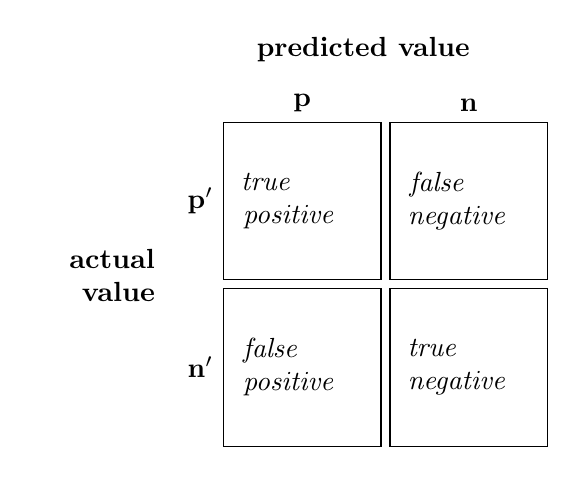
\begin{tikzpicture}[
box/.style={draw,rectangle,minimum size=2cm,text width=1.5cm,align=left}]
\matrix (conmat) [row sep=.1cm,column sep=.1cm] {
\node (tpos) [box,
    label=left:\( \mathbf{p'} \),
    label=above:\( \mathbf{p} \),
    ] {\textit{true} \\ \textit{positive}};
&
\node (fneg) [box,
    label=above:\textbf{n},
    ] {\textit{false} \\ \textit{negative}};
\\
\node (fpos) [box,
    label=left:\( \mathbf{n'} \),
    label=below left:,
    ] {\textit{false} \\ \textit{positive}};
&
\node (tneg) [box,
    ] {\textit{true} \\ \textit{negative}};
\\
};
\node [left=.05cm of conmat,text width=1.5cm,align=right] {\textbf{actual \\ value}};
\node [above=.05cm of conmat] {\textbf{predicted value}};
\end{tikzpicture}
\end{center}
\caption{A confusion matrix defining the four outcomes of classification. In the previous example of e-mail/spam classification, labeling a spam e-mail as spam results in a \textit{true positive}; labeling a non-spam e-mail as spam results in a \textit{false positive}; labeling a spam e-mail as not spam results in a \textit{false negative}; labeling a non-spam e-mail as not spam results in a \textit{true negative}.}
\end{figure}

\subsection{State-of-the-art machine learning algorithms}
As exaplained by Wolpert's ``no free lunch'' theorem \cite{wolpert1995}, machine learning algorithms cannot be evaluated in a vaccuum; their performance must always be characterized with respect to a specific application whose test data are clearly defined. This limitation makes it impossible to provide an absolute ranking of existing machine learning techniques; a given algorithm that performs well in one context may perform terribly in another. Nonetheless, researchers have conducted empirical studies in order to compare the performance of different algorithms; some are consistently more powerful than others, including neural nets, support-vector machines (SVMs), and bagged trees \cite{caruana2006}. In medical informatics, the choice of a machine learning strategy is often constrained by characteristics of both medical data and the clinical environment, some of which are discussed below.



%------------------------------------------------
\section{Machine learning challenges in medical informatics}
\subsection{Class imbalance and asymmetric costs}
Supervised learning algorithms perform best when the training data contains approximately equal quantities of the classes (e.g., a corpus of e-mail messages, half of which is spam, half of which is not). The performance degrades, however, if a ``class imbalance'' exists in the training data \cite{guo2008, he2009}. Depending on the domain, class imbalance can be either relatively minor (e.g., 10:1) or very severe (e.g., 10000:1) \cite{he2009}. A common application of machine learning in medical informatics is in the classification of disease states. In such cases, training instances in which the disease is present are given the positive label, and instances in which the disease is absent are given the negative label. It is often the case, however, that there are far fewer people in a population with a certain disease than those without it. Therefore, data sets that are produced from research on such populations will yield far more negative instances than positive ones.

Training an algorithm with imbalanced data leads to poor sensitivity, because---given the overabundance of one of the classes---the training process tends to produce a classifier that is biased toward the majority class \cite{guo2008}. This in turn leads to a high occurrence of false negatives \cite{wallace2012}. Note in Equation \ref{eq:sensitivity} that raising the value of \textit{FN} will result in a larger denominator, and therefore a lower value for sensitivity. Although the above strategies can be effective, imbalanced data sets present further complications when the costs associated with false positives and false negatives are unequal.

The cost or penalty of making a false positive prediction is not always equal to the cost or penalty of making a false negative prediction.
This fact further complicates training with imbalanced data sets, because additional considerations must be made regarding the biases that may result in the classifier.
This problem is especially challenging when researchers are most interested in correctly classifying the minority class, and when the cost of low sensitivity toward the minority class is high \cite{wallace2012}.

\subsubsection{Strategies for addressing class imbalance}
Guo, et al. \cite{guo2008} categorize strategies for mitigating class imbalance into four groups, each of which corresponds to a different part of the machine learning process.
The first (and perhaps simplest) method is to sample the training instances to achieve greater class balance.
This can be achieved by either under-sampling the majority class, over-sampling the minority class, or some combination of the two.
Despite the simplicity of this approach, it has been shown to be quite effective under certain conditions \cite{japkowicz2000}.
The second method is to perform feature selection, which is a strategy for eliminating irrelevant and redundant features from the training data.
The third method is to bias the classier directly to counteract the bias that would occur otherwise due to class imbalance.
The fourth and final method is to employ ensemble learning, which combines the output of multiple classifiers according to task-specific rules; examples of this strategy are boosting and bagging \cite{guo2008}.


\subsection{Scarcity of domain experts, abundance of data}
The development of machine learning algorithms is often informed by experts from the domain in which the algorithms will be applied. When applying machine learning techniques to a specific field, researchers must often make considerable use of domain experts' knowledge to inform both the design of algorithms and the correct labels for training data.
This holds true when machine learning is applied to medical informatics.
A problem, though, is that the domain experts in medical informatics---physicians and other caregivers---are often extremely busy, and thus unable to participate in some of the labor-intensive, time-consuming tasks that can accompany scientific research.
Therefore, the ability of machine learning algorithms to automate various clinical and research tasks holds great promise for physicians who lack sufficient time to complete them. Additionally, when a physician's input is required to inform machine learning work---for example, when screening data sets for algorithm training---advanced machine learning techniques can help to minimize the amount of time the physician needs to dedicate to the training process \cite{wallace2012}.

One of the most illustrative examples of such a task is the systematic review, in which an exhaustive search of the clinical literature is performed in order to answer a specific medical question \cite{counsell1997}. These reviews commonly require trained personnel to review thousands of abstracts to ensure that relevant articles are not excluded arbitrarily from the analysis \cite{wallace2012}. Specific machine learning methods can leverage expertise in order to minimize the amount of time that domain experts need to be involved in a task. The following sections present various ways in which medical domain experts can augment machine learning work, as well as machine learning's positive effects on physicians' work.


\subsubsection{Strategies for addressing the scarcity of domain experts}
\textit{Dual supervision} is a machine learning strategy in which ``domain expert(s) provide explicit information regarding features and their relationship to class labels'' \cite{wallace2012}.
Dual supervision can reduce the amount of work that experts must perform, because, in certain cases, providing additional knowledge about the features is more effective than traditional supervised learning algorithms.
Rather than learning certain relationships over the course of numerous training instances, specific aspects of the model (e.g., classifier) are informed directly by an expert.
To the extent that dual supervision lessens the requirement for training instances, fewer training data require manual labeling, thereby reducing the time commitment required of experts during training. For example, a physician who has years of experience in the pathology of cancer can convey this knowledge to a classifier by annotating features in a data set in a machine-readable format.

\textit{Active learning} is another strategy for reducing various costs associated with training.
An assumption of active learning is that an algorithm can be trained more efficiently if the training data is selected strategically.
This selection process usually occurs via \textit{queries} that are submitted to an \textit{oracle}, which is generally a human expert who can provide the correct label of a given training instance \cite{settles2009}.
Queries can even result in the creation of new training instances that did not appear in the original data set \cite{angluin1987}.
A problem with active learning is that it generally assumes that its oracle will provide perfectly accurate labels for all queries, and that it will do so for a constant cost; this assumption is simply false in many cases \cite{wallace2012}.

\textit{Dually-supervised active learning} combines the previous two approaches and makes use of labeled features (from dual supervision) in an active learning framework. Empirical tests have shown that this strategy is particularly useful for training on data sets with significant class imbalance \cite{wallace2012}. Because of its efficient use of domain experts and its accommodation of class imbalance, dually-supervised active learning techniques show great promise for applications in medical informatics. As discussed below, they may also help physicians who interact with machine learning systems to feel more confident in classifiers' results.


%------------------------------------------------


\section{Future directions}
When machine learning is applied to medical informatics, two kinds of expertise are involved: that of the physicians who understand the given feature space, and that of the computer scientists who design the algorithms in light of the physicians' input. The success of this process depends on how well each group can present their knowledge in a way that is understandable by the other. Recent efforts have been made to close this loop more robustly---that is, to give domain experts the ability to interact with the data in a way that both imparts their expertise and directly impacts the resulting machine learning parameters that are used \cite{brown2012, liu2011}. Such advances are ingenious in that they drastically improve a physicians' ability to improve the training of algorithms directly, as well as providing an intuitive strategy for doing so. One can envision many clinical applications of these interactive technologies, including improved clinical decision support systems. If physicians are given greater and more direct control over the machine learning algorithms, they may have a better intuition for how their domain knowledge constrains the algorithm's design, and may therefore have greater confidence in the output of such systems.
%------------------------------------------------



%------------------------------------------------
\section{Conclusion}
It was reported in \cite{miliard2013} that, according to a recent IDC Health Insights survey, almost 60 percent of physicians in ambulatory care settings are unsatisifed with EHRs because of the negative effects they have on clinical workflows.
It is clear from such statistics such as this that physicians' clinical interactions with machines need to change considerably before there is unanimous agreement that computers are aids---and not obstacles---in healthcare.
Machine learning techniques hold great promise for expediting time-consuming research tasks and for automating overwhelmingly large data mining tasks---in short, for making physicians' lives easier.

One way to frame this relationship is that machine learning techniques afford physicians the ability to embed a part of their expertise in the computing systems that surround them, rather than always having to be a point of contact in the transmission of such information.
Machines that have ``learned'' from a physician's experience can continue to benefit others who utilize the resulting model, and subsequent uses of these algorithms do not require repetitive input from the physician.
Methods such as dually supervised active learning and interactive training visualizations continue to minimize the effort required of physicians to impart their knowledge to classifiers.
In addition to developing increasingly robust training methods, machine learning researchers would do well to develop interfaces that give non-computer scientists a better intuition for  the machine learning workflow, including methods for mapping the parameters of an algorithm to their clinical meaning or significance.

%------------------------------------------------



%----------------------------------------------------------------------------------------
%	BIBLIOGRAPHY
%----------------------------------------------------------------------------------------
\newpage
\bibliographystyle{plain}
\bibliography{m227_project_2}
%----------------------------------------------------------------------------------------

\end{document}
